\documentclass{standalone}

\usepackage{standalone}
\usepackage{tikz}
\usetikzlibrary{calc,intersections}

\begin{document}
	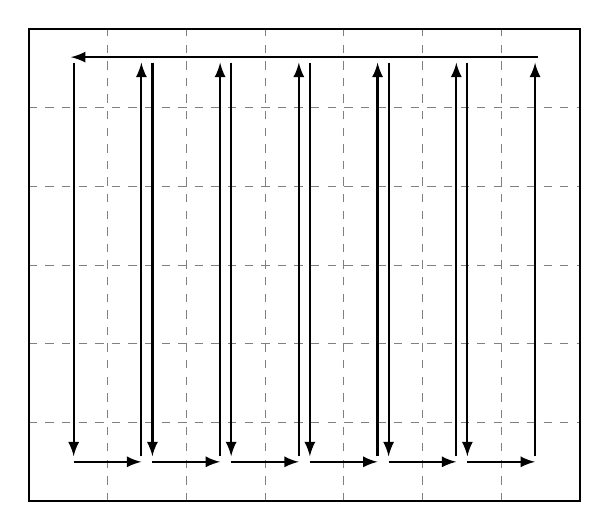
\begin{tikzpicture}
	
		\pgfmathtruncatemacro{\xsize}{7}
		\pgfmathtruncatemacro{\ysize}{6}


		\pgfmathsetmacro{\arrowoffset}{0.07}
		\draw[dashed, very thin, black!50] (0,0) grid (\xsize, \ysize);
		\draw[thick] (0, 0) --
			(0, \ysize) --
			(\xsize, \ysize) --
			(\xsize, 0) --
			cycle;

		\pgfmathtruncatemacro{\xinnersize}{\xsize - 2}
		\pgfmathtruncatemacro{\yinnersize}{\ysize - 2}
		
		\begin{scope}[shift={(0.5, 0.5)}, thick]
			\foreach \col in {0, ..., \xinnersize}
			{
				\draw[-latex] (\col + \arrowoffset, \yinnersize + \arrowoffset + 1) -- (\col + \arrowoffset, \arrowoffset); % arrow down
				\draw[-latex] (\col + 1 - \arrowoffset, \arrowoffset) -- (\col + 1 - \arrowoffset, \yinnersize + 1 + \arrowoffset); % arrow up

				\draw[-latex] (\col + \arrowoffset, 0) -- (\col + 1 - \arrowoffset, 0); % arrow right
			}
			\draw[-latex] (\xinnersize + 1 - 0.5 * \arrowoffset, \yinnersize + 1 + 2 * \arrowoffset) -- (0 + 0.5 * \arrowoffset, \yinnersize + 1 + 2 * \arrowoffset); % arrow left
		\end{scope}
	\end{tikzpicture}
\end{document}
